\chapter{Implementasi dan Pengujian}
Bab ini akan menjelaskan proses implementasi dari rancangan solusi yang telah dikaji pada Bab III. Setelah pembahasan terkait implementasi, akan dilanjutkan dengan pemaparan hasil uji terkait implementasi yang telah dibuat.

\section{Lingkungan}

\textit{Autoscaler} berbasis kontrol fleksibel akan diimplementasikan di lingkungan komputer lokal. Berikut adalah lingkungan perangkat keras dan perangkat lunak secara terperinci.

Implementasi sistem tugas akhir dilakukan dengan mengimplementasikan dengan bantuan beberapa kakas pada bahasa \textit{python}. Sistem akan hidup di luar \textit{kubernetes cluster} dan mengakses Kubernetes beserta \textit{pods}-nya melalui \textit{Kubernetes Client Library} dan \textit{service Elastic search} melalui \textit{web service} yang dapat diakses dari luar \textit{cluster}.

\textit{Autoscaler} berbasis kontrol fleksibel akan berjalan di \textit{cluster} Kubernetes lokal. Adapun spesifikasi dari komputer yang dipakai untuk pengembangan adalah sebagai berikut.
\begin{enumerate}
    \item \textbf{Perangkat Keras}
    
        \begin{enumerate}
            \item CPU: \textit{Apple M1 Chip}
            \item RAM: 16 GB
        \end{enumerate}
    
    \item \textbf{Perangkat Lunak}
        
        \begin{enumerate}
            \item Platform dan Sistem Operasi: Darwin AMD64, MacOS Monterey 12.6
            \item \textit{Containerization}: Docker
            \item \textit{Kubernetes Cluster}:
                \begin{enumerate}
                    \item Kubernetes Client v1.27.1-eks-2f008fe
                    \item Kubernetes Docker Desktop: Kubernetes v1.25.9
                \end{enumerate}
            \item Bahasa: Python 3.9.12
            \item Dependensi Lain:
                \begin{enumerate}
                    \item \textit{Kubernetes Client Library}
                    \item \textit{Pandas, numpy, statsmodels dan pmdarima}
                    \item \textit{Pickle}
                \end{enumerate}
        \end{enumerate}
\end{enumerate}

\section{Implementasi}

Bagian ini akan menjelaskan tentang implementasi sistem kontrol adaptif secara terperinci.

\subsection{Batasan Implementasi}
Berikut adalah batasan yang ditetapkan dalam melakukan implementasi sistem kontrol adaptif.
\begin{enumerate}
    \item Masih menerapkan sistem \textit{single node} dan \textit{single pod}.
    \item Tidak memperhatikan optimalisasi dari model ARIMA.
    \item Hanya dapat menangani \textit{metrics} yang sudah ditentukan, yaitu \textit{throughput} dari setiap operasi \textit{Elastic Search} serta utilisasi prosesor hingga memori.
    \item Tidak mempertimbangkan besarnya model seiring bertambahnya data.
    \item Komponen \textit{Metrics Fetcher} berjalan di proses lain dan diimplementasikan dalam \textit{script} yang berbeda dikarenakan bahasa Python memiliki kekurangan dalam penanganan \textit{multithreading}.
    \item Pertukaran data antara komponen \textit{Metrics Fetcher} dan \textit{Predictor} melalui stream file.
\end{enumerate}

\subsection{Kakas yang Digunakan}
Dalam melakukan implementasi ini diperlukan beberapa kakas, diantaranya adalah sebagai berikut.
\begin{enumerate}
    \item \textit{Docker}, \textit{Docker Desktop} dan \textit{Docker Desktop Kubernetes} untuk dipakai sebagai \textit{containerization} dan \textit{cluster} kubernetes lokal.
    \item Minikube dipakai sebagai \textit{cluster} kubernetes lokal dengan versi yang lebih baru karena versi \textit{Docker Desktop Kubernetes} hanya memakai yang \textit{stable} dan tidak bisa dipaksa naik versi.
    \item Pandas dan Numpy untuk keperluan \textit{data processing} serta bentuk data untuk dikirimkan ke komponen lain serta model prediksi ARIMA.
    \item \textit{Kubernetes Python Client} untuk mengontrol \textit{cluster} kubernetes melalui kode Python.
    \item \textit{Pickle} untuk menyimpan model ARIMA sehingga persisten meskipun sistem di-\textit{restart}.
    \item \textit{Statsmodels} dan \textit{pmdarima} untuk membangun model ARIMA serta melakukan otomasi pencarian orde atau lebih dikenal sebagai Auto-ARIMA.
\end{enumerate}

% TODO Untuk spesifikasi pods 

\subsection{Sistem Kontrol Adaptif dengan Model Prediktif berbasis \textit{Time Series}}

Seperti yang sudah dijelaskan pada bagian rancangan solusi (\ref{sec:rancangan-solusi}), sistem kontrol adaptif akan diimplementasikan dengan beberapa komponen penyusun, diantaranya adalah sebagai berikut.

% TODO \subsubsection{Tampilan Implementasi}

\subsection{Eksperimen \textit{In-place Resource Resize} untuk \textit{pods Kubernetes}}

Pada bagian sebelumnya, diperlukan \textit{resizing} sumber daya yang dialokasikan untuk \textit{pods} yang sedang berjalan tanpa melakukan \textit{restart}. Untuk hal tersebut, perlu dilakukan eksperimen, berikut adalah rincian dari eksperimen yang telah dilakukan.

\subsubsection{Pendahuluan}

\textit{In-place Resource Resize} adalah fitur untuk mengubah ukuran sumber daya CPU dan memori yang dialokasikan untuk kontainer pada pod yang sedang berjalan tanpa harus me-\textit{restart} pod atau kontainernya. Sebuah \textit{node} Kubernetes mengalokasikan sumber daya untuk sebuah pod berdasarkan permintaannya, dan membatasi penggunaan sumber daya pod berdasarkan batasan yang ditentukan dalam kontainer-kontainer pod tersebut. Fitur ini baru hadir pada versi Kubernetes 1.27.0, dan, pada saat tugas akhir ini dikerjakan, masih dalam tahap \textit{alpha testing} dan pengembangan. Berdasarkan \parencite{kubeinplaceupdate2}, dokumentasi resmi dipublikasikan pada 30 Maret 2023 7:59 PM PST. Sedangkan berdasarkan \parencite{kubeinplaceupdate}, publikasi \textit{alpha testing} semenjak 13 Mei 2023.

\subsubsection{Pengerjaan Eksperimen}
Dalam melakukan eksperimen ini, dilakukan beberapa tahap sebagai berikut.

\begin{enumerate}
    \item Memastikan versi Kubernetes yang digunakan adalah versi 1.27.0 atau lebih baru pada \textit{client} dan \textit{server}.
    
    Pada saat itu, Kubernetes lokal yang dipakai adalah \textit{Docker Desktop Kubernetes} yang membatasi versi Kubernetes pada versi 1.25.9. Sehingga, dilakukan pengubahan server dengan menggunakan Minikube. Sayangnya, versi maksimal yang bisa dipakai oleh Minikube adalah Kubernetes versi 1.27.0-rc0, versi 1.27 yang paling pertama atau \textit{release candidate 0}. Untuk mengecek bisa dilihat pada \url{https://github.com/kubernetes/minikube/releases/tag/v1.30.0}. Dicoba juga untuk dipaksa menggunakan versi 1.27.1 maupun 1.27.3, namun hal tersebut gagal untuk dilakukan. Sehingga, untuk eksperimen ini, digunakan Kubernetes versi 1.27.0-rc0 melalui Minikube.

    \item Membuat \textit{deployment} yang akan digunakan untuk eksperimen.
    
    Konfigurasi \textit{deployment} berubah, karena untuk menggunakan fitur ini, tidak bisa membuat \textit{pods} dengan menggunakan tipe \textit{deployment} melainkan harus langsung membuat dengan tipe \textit{pod}. Terdapat juga beberapa konfigurasi baru yang perlu diatur.

    \item Mengeksekusi perintah untuk melakukan \textit{in-place resource resize}.
    
    Hal ini bisa dilakukan dengan mengeksekusi perintah \textit{patch pod}. Perintah ini bisa dilihat pada dokumentasi: \url{https://kubernetes.io/docs/tasks/configure-pod-container/resize-container-resources/}.

    Saat hal ini dijalankan terdapat pesan eror yang mengatakan bahwa fitur \textit{patch} tersebut hanya bisa dilakukan selain resource. Padahal, inisiasi eksperimen sudah disesuaikan dengan \textit{requirement} yang disebutkan pada dokumentasi.

    \item Mengecek detail informasi \textit{pods}
    
    Seharusnya, ketika mengecek detail informasi \textit{pods} akan terlihat bahwa resource yang digunakan sudah berubah dan terdapat informasi-informasi baru yang hanya muncul pada versi terbaru Kubernetes. Namun, hal ini tidak terjadi. Resource yang digunakan masih sama dengan sebelumnya. Dan hasil detail informasi sebuah \textit{pods} tidak memperlihatkan detail informasi terbaru yang sesuai dengan contoh pada dokumentasi.
\end{enumerate}

\subsubsection{Hasil Eksperimen}

Berdasarkan hasil eksperimen tersebut, dapat disimpulkan bahwa.

\begin{enumerate}
    \item Fitur \textit{in-place resource resize} belum bisa digunakan pada Kubernetes versi 1.27.0-rc0.
    \item Melakukan \textit{resource resize} tanpa melakukan \textit{restart} mungkin bisa dilakukan pada masa yang akan datang.
    \item Eksperimen ini bisa dicoba lagi pada masa yang akan datang. Mengingat tools kubernetes lokal masih belum bisa menggunakan versi \textit{alpha} terbaru. Dan, pada saat ini, fitur ini masih dalam tahap \textit{alpha testing} dan pengembangan.
\end{enumerate}

Sehingga, untuk saat ini, eksperimen ini tidak bisa dilakukan lebih jauh lagi. Dan oleh karena itu, sistem kontrol adaptif yang dibuat masih memakai sistem \textit{Rolling Update} untuk mengubah sumber daya alokasi. Namun, kedepannya, jika ingin diteruskan, besar kemungkinan hal ini bisa dilakukan karena dari Kubernetes sendiri sedang mengembangkan fitur tersebut.

\section{Pengujian}

Bagian ini akan menjelaskan beberapa skenario yang dilakukan untuk menguji sistem kontrol adaptif. Pengujian akan dilakukan per komponen lalu dilanjutkan dengan satu sistem penuh. Setiap skenario pengujian akan dijelaskan tujuannya, skenario yang dilakukan, dan hasil pengujian yang didapatkan.

% \subsection{Pengujian X}

% \subsubsection{Tujuan Pengujian}

% \subsubsection{Skenario Pengujian}

% \subsubsection{Hasil Pengujian dan Analisis}

\subsection{Pengujian Komponen \textit{Metrics Fetcher}}

Pada bagian ini akan dijelaskan tentang tujuan, skenario, hasil, dan analisis dari pengujian komponen \textbf{\textit{Metrics Fetcher}}.

\subsubsection{Tujuan Pengujian}

Tujuan pengujian ini memastikan komponen \textbf{\textit{Metrics Fetcher}} dapat berjalan dengan baik dan menghasilkan data yang sesuai dengan ekspektasi.

\subsubsection{Skenario Pengujian}

Pengujian terhadap komponen \textbf{\textit{Metrics Fetcher}} dilakukan dengan beberapa skenario sebagai berikut serta ekspektasi dari pengujian yang dilakukan.
\begin{enumerate}
    \item \textit{Elastic Search} sedang \textit{idle}.
        Data yang diminta dari \textit{Node Stats API} diekspektasikan relatif statis dan berhasil diletakkan pada \textit{stream file}.
    \item \textit{Elastic Search} sedang digunakan untuk melakukan operasi penambahan data.
        Data yang diminta dari \textit{Node Stats API} seharusnya relatif berubah terutama pada aspek \textit{throughput} operasi \textit{index} dan \textit{bulk}. Lalu, data tersebut diekspektasikan berhasil diletakkan pada \textit{stream file}.
    \item \textit{Elastic Search} sedang digunakan untuk melakukan operasi pencarian data.
        Data yang diminta dari \textit{Node Stats API} seharusnya relatif berubah terutama pada aspek \textit{throughput} operasi \textit{query} dan \textit{fetch}. Lalu, data tersebut diekspektasikan berhasil diletakkan pada \textit{stream file}.
\end{enumerate}

\subsubsection{Hasil Pengujian dan Analisis}

Hasil untuk skenario 1 dapat dilihat pada gambar \ref{fig:mf-1}. Data yang ditarik sudah relatif statis untuk semua aspek dan berhasil diletakkan pada \textit{stream file}. Untuk skenario 2, dapat dilihat pada gambar \ref{fig:mf-2}. Data yang ditarik sudah mengalami perubahan pada operasi \textit{index} dan \textit{bulk} serta berhasil diletakkan pada \textit{stream file}. Terakhir, skenario 3, dapat dilihat pada gambar \ref{fig:mf-3}. Data yang ditarik sudah mengalami perubahan pada operasi \textit{query} dan \textit{fetch} serta berhasil diletakkan pada \textit{stream file}.

\begin{figure}[h]
    \centering
    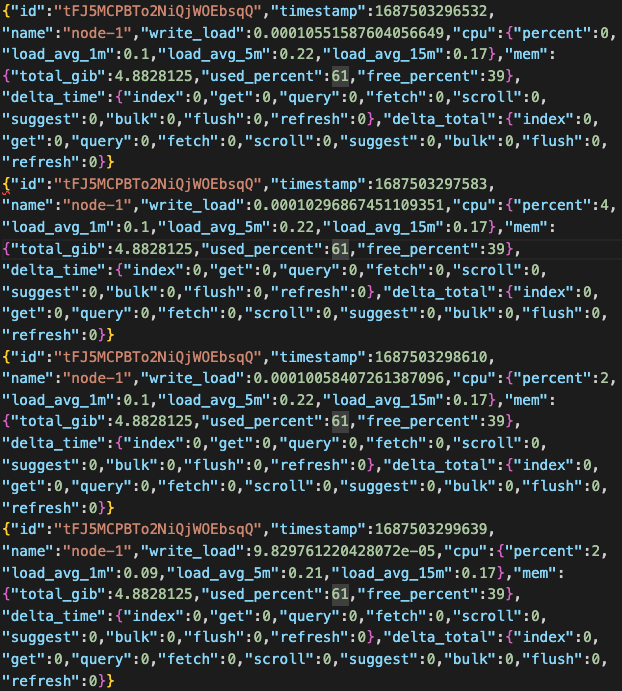
\includegraphics[width=0.8\textwidth]{chapter-4/mf-1.png}
    \caption{Hasil Pengujian Komponen \textit{Metrics Fetcher} Skenario 1}
    \label{fig:mf-1}
\end{figure}

\begin{figure}[h]
    \centering
    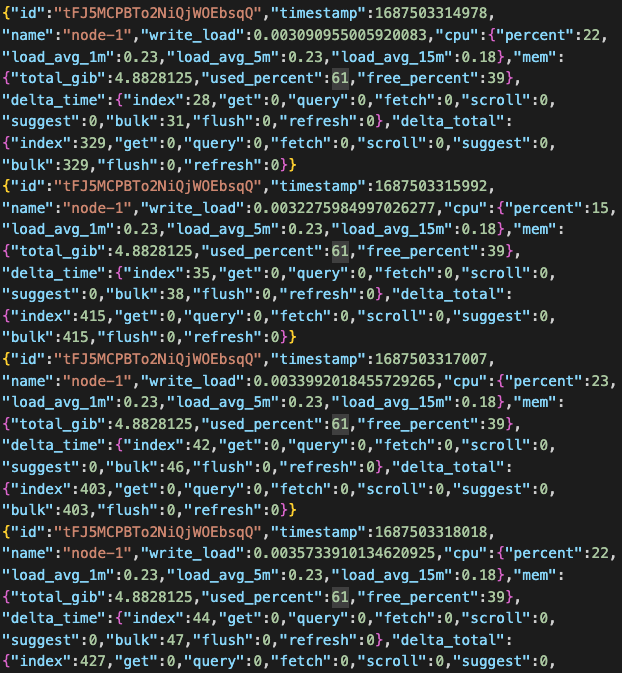
\includegraphics[width=0.8\textwidth]{chapter-4/mf-2.png}
    \caption{Hasil Pengujian Komponen \textit{Metrics Fetcher} Skenario 2}
    \label{fig:mf-2}
\end{figure}

\begin{figure}[h]
    \centering
    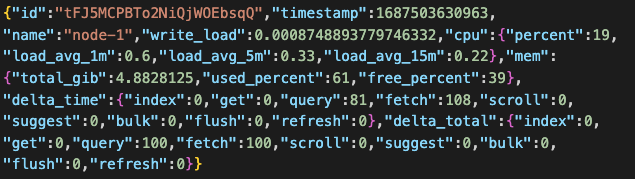
\includegraphics[width=0.8\textwidth]{chapter-4/mf-3.png}
    \caption{Hasil Pengujian Komponen \textit{Metrics Fetcher} Skenario 3}
    \label{fig:mf-3}
\end{figure}

Maka untuk pengujian komponen \textbf{\textit{Metrics Fetcher}} sudah sesuai ekspektasi dan dapat dilanjutkan ke pengujian komponen lainnya.
\subsection{Pengujian Komponen \textit{Rule Manager}}
\subsection{Pengujian Komponen \textit{Predictor}}
\subsection{Pengujian Komponen \textit{Resource Controller}}
\subsection{Pengujian Sistem \textit{Adaptive Control}}

Pada bagian ini akan dijelaskan tentang tujuan, skenario, hasil, dan analisis dari pengujian sistem sekaligus komponen \textbf{\textit{Adaptive Control}}.

\subsubsection{Tujuan Pengujian}

Tujuan pengujian ini memastikan sistem \textbf{\textit{Metrics Fetcher}} dapat berjalan dengan baik dan menghasilkan perilaku yang sesuai.

\subsubsection{Skenario Pengujian}

Pengujian terhadap komponen \textbf{\textit{Metrics Fetcher}} dilakukan dengan beberapa skenario sebagai berikut serta ekspektasi dari pengujian yang dilakukan.
\begin{enumerate}
    \item Sebuah \textit{rule} memenuhi kondisi untuk mengubah alokasi prosesor.
    
    Prosesor akan berubah jumlahnya sesuai dengan \textit{rule} yang memenuhi kondisi. Perubahan pada spesifikasi \textit{pods} juga diekspektasikan mengikuti.

    \item Sebuah \textit{rule} memenuhi kondisi untuk mengubah alokasi memori.
    
    Prosesor akan berubah jumlahnya sesuai dengan \textit{rule} yang memenuhi kondisi. Perubahan pada spesifikasi \textit{pods} juga diekspektasikan mengikuti. Memory Used Percent akan menurun karena penambahan yang terjadi.
\end{enumerate}

\subsubsection{Hasil Pengujian dan Analisis}

Pengujian akan dilakukan dengan \textit{file rule} yang dapat dilihat pada gambar \ref{fig:ac-rule}. Terdapat dua buah \textit{rule} yang akan diuraikan sebagai berikut.

\begin{enumerate}
    \item Jika \textit{load average 1m} pada 10 detik kedepan diprediksikan diatas 0 maka akan ditambah alokasi prosesor sebesar 1000m atau sejumlah 1. Sebagai catatan, kondisi dari \textit{rule} dibuat agar rule pasti terpenuhi.
    \item Jika \textit{memory used percent} pada 5 dan 10 detik kedepan diprediksikan diatas 60 maka akan ditambah alokasi memori sebesar 2048 mebibyte atau sejumlah 2 gibibyte (Gi). Sebagai catatan, kondisi dari \textit{rule} dibuat agar rule pasti terpenuhi.
\end{enumerate}

Hasil dari pengujian skenario kedua dapat dilihat pada gambar \ref{fig:ac-mem}. Dan perubahan terhadap spesifikasi pods dapat dilihat pada gambar \ref{fig:ac-mem-kube}. Perubahan juga terjadi pada \textit{memory used percent} pada \textit{stream file} atau data yang ditarik oleh komponen \textbf{\textit{Metrics Fetcher}} dapat dilihat pada gambar \ref{fig:ac-mf-turun}.
Diikuti dengan hasil dari pengujian skenario pertama dapat dilihat pada gambar \ref{fig:ac-cpu}. Dapat dilihat bahwa prosesor berubah sesuai dengan ekspektasi. Perubahan pada spesifikasi \textit{pods} juga mengikuti perubahan prosesor yang dapat dilihat pada gambar \ref{fig:ac-cpu-kube}.

\begin{figure}[h]
    \centering
    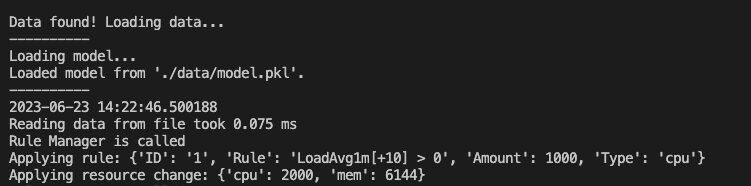
\includegraphics[width=0.8\textwidth]{chapter-4/ac-cpu.png}
    \caption{Hasil Pengujian Komponen \textit{Adaptive Control} Skenario 1: Perubahan Prosesor}
    \label{fig:ac-cpu}
\end{figure}

\begin{figure}[h]
    \centering
    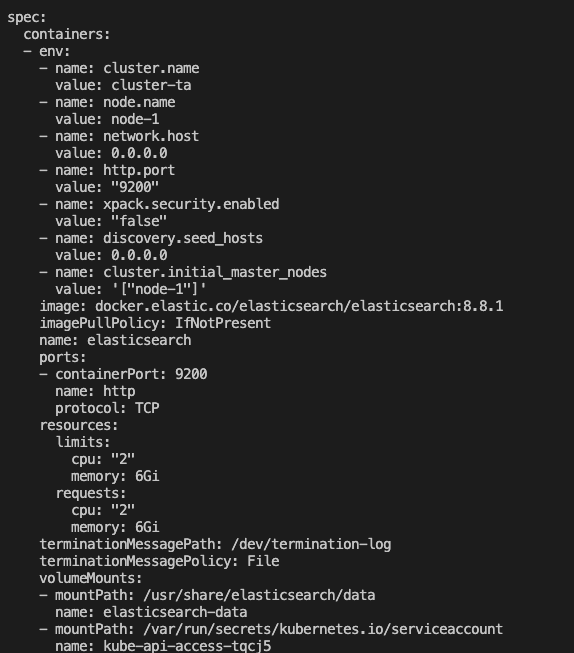
\includegraphics[width=0.8\textwidth]{chapter-4/ac-cpu-kube.png}
    \caption{Hasil Pengujian Komponen \textit{Adaptive Control} Skenario 1: Perubahan Spesifikasi Kubernetes}
    \label{fig:ac-cpu-kube}
\end{figure}

\begin{figure}[h]
    \centering
    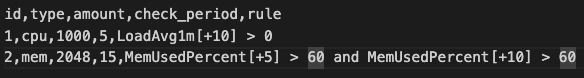
\includegraphics[width=0.8\textwidth]{chapter-4/ac-rule.png}
    \caption{File Rule untuk Pengujian Komponen \textit{Adaptive Control}}
    \label{fig:ac-rule}
\end{figure}

\begin{figure}[h]
    \centering
    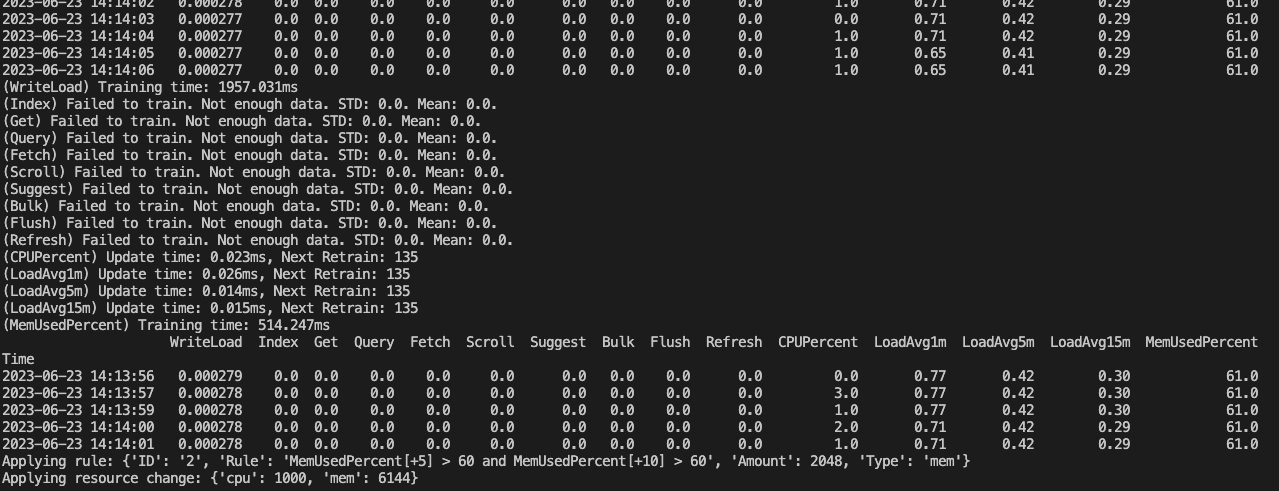
\includegraphics[width=0.8\textwidth]{chapter-4/ac-mem.png}
    \caption{Hasil Pengujian Komponen \textit{Adaptive Control} Skenario 2: Perubahan Memori}
    \label{fig:ac-mem}
\end{figure}

\begin{figure}[h]
    \centering
    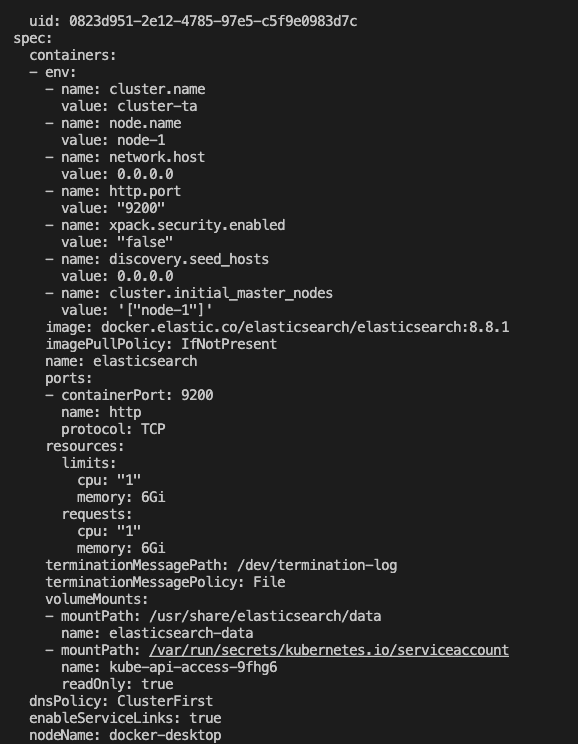
\includegraphics[width=0.8\textwidth]{chapter-4/ac-mem-kube.png}
    \caption{Hasil Pengujian Komponen \textit{Adaptive Control} Skenario 2: Perubahan Spesifikasi Kubernetes}
    \label{fig:ac-mem-kube}
\end{figure}

\begin{figure}[h]
    \centering
    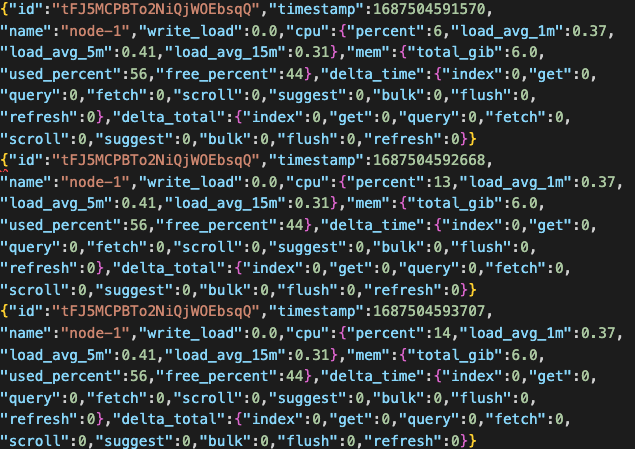
\includegraphics[width=0.8\textwidth]{chapter-4/ac-mf-turun.png}
    \caption{Hasil Pengujian Komponen \textit{Adaptive Control} Skenario 2: Perubahan Memory Used Percent pada \textit{stream file}}
    \label{fig:ac-mf-turun}
\end{figure}

Maka untuk pengujian komponen \textbf{\textit{Adaptive Control}} sudah sesuai ekspektasi dan sistem dapat berjalan dengan baik.